\DiaryEntry{Breadth-First Search (UPdate 2020-10-12)}{2020-02-24}{Algorithms}

We have a graph $G$ with vertex set $V$ and edge set $E$ and a source vertex $s$. Breadth-first starts at $s$ and systematically walks along the graph edges to visit each vertex. During this walk, it produces two results ``on the way'',

\begin{itemize}
\item It calculates the distance (smallest number of edges) from $s$ to every vertex. If a vertex is not reachable from $s$, the distance is $\infty$.
\item It produces a breadth-first tree with root $s$ that contains all reachable vertices.
\item It stores the parent vertex of each vertex.
\end{itemize}

The algorithm is called breadth-first because it advances uniformly across the breadth of the frontier. A depth-first algorithm digs to the leaves of the tree first.

The algorithm keeps track of progress by assigning a different cvolor to each vertex as follows

\begin{itemize}
\item Initially, all vertices are colored \emph{white}.
\item If a vertex is discovered, its color becomes non-white. Gray and black vertices, have been discovered; their difference is as follows
  \begin{itemize}
  \item If a vertex $v$ is black, then a neighbouring vertex $u$ with $(u,v) \in G$ is non-white.
  \item A grey vertex may have some adjacent white vertices. The color grey therefore represents the frontier between discovered and undiscovered vertices.
  \end{itemize}
\end{itemize}

The algorithm stores the vertex color, parent, and distance in additional attributes of a vertex. In addition, the algorithm uses a queue Q wich works in a first-in first-out fashion. It is this queue which enforces the breadth-first characteristic.

In pseudo-code, the algorithm looks as follows

\begin{Verbatim}[numbers=left, xleftmargin=5mm]
BFS(G,s)
for each vertex u in G:V -s
   u.color = WHITE
   u.d = 1
   u.parent = NULL
s.color = GRAY
s.d = 0
s.parent = NULL
enqueue(Q,s)
while Q is non-empty
   u = dequeue(Q)
   for each v in adjacent(G,u)
      if v.color == WHITE
         v.color = GRAY
         v.d = u.d + 1
         v.parent = u
         enqueue(Q,v)
   u.color = BLACK
\end{Verbatim}

Lines 2 - 5 initialize all vertices. Lines 6 - 8 mark the source vertex as grey and enqueue it in Q (line 9). Then the algorithm works on the queued items (line 10): It takes a vertex u from the queue (line 11) and proceeds with its neighbours (line 12). If the vertex is white; i.e. has not been visited (line 13), it colors the vertex gray, updates distance and parent (lines 14 - 16) and enqueues it (line 17). Finally, it marks u as black.

The check whether a vertex is white (line 13) prevents considering a vertex twice (and therefore introducing loops).

The results provided by the BFS depend (of course) on the starting vertex. In addition, the same graph can have different order of vertices in the adjacency matrix (which is used in e.g. line 12), which may result in different parent attributes. The distances calculated will be same.

Cormen et al contains some proofs that the breadth-first algorithm does what it is supposed to do; we skip that here. What is interesting, though, is a procedure to extract the path from a certain vertex $v$ to the root vertex $s$. Starting at vertex $v$, the algorithm goes ``up'' along v.parent until (i) it has reached $s$, or (ii) when the vertex has no parent. In the latter case, there is no path between $s$ and $v$.

\begin{verbatim}
print-path(G,s,v)
   if v == s
      print s
   else if v.parent = NULL
      print "no path"
   else
      print-path(G,s,v.parent)
      print v
\end{verbatim}

We finally note that Julia provides the LightGraph package which has an BFS implementation; for the example from Cormen, see \href{https://github.com/ClemensFMN/JuliaStuff/blob/master/Graphs/bfs_traversal.jl}{this file}.

\paragraph{Example.} As an example, we consider the graph shown in the following Figure.

\begin{figure}[H]
   \centering
   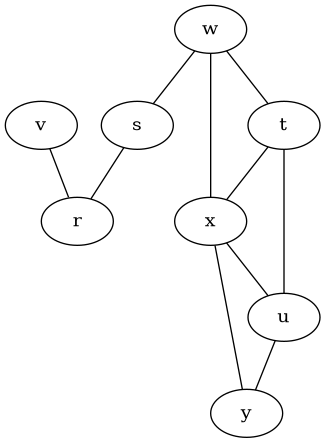
\includegraphics[scale=0.5]{images/graphs_bst_01.png}
\end{figure}

In the following, we execute the BFS algorithm and output the queue \verb Q  before the dequeuing in line $11$ and the element \verb u which is dequeued in line $11$. We start the algorithm with vertex \verb s , so 

\begin{verbatim}
   Q =[s]
   u = s
\end{verbatim}

The algorithm enqueues the two neighbours of \verb s  which are \verb r  and \verb w . It continues by taking vertex \verb r  from the queue. 

\begin{verbatim}
   Q =[r, w]
   u = r
\end{verbatim}

Having visited vertex \verb r  , it pushes the neighbouring vertex \verb v  to the queue and continues with vertex \verb w .

\begin{verbatim}
   Q =[w, v]
   u = w
\end{verbatim}

The unvisited neighbours of \verb w  are vertices \verb x  and \verb t  which are added to the queue. The algorithm takes vertex \verb v  from the queue.

\begin{verbatim}
   Q =[v, x, t]
   u = v
\end{verbatim}

Since vertex \verb v  has no unvisited neighbours, no new vertices are added and the algorithm continues with vertex \verb v  (although nothing happens).

\begin{verbatim}
   Q =[x, t]
   u = x
\end{verbatim}

Now the algorithm continues with vertex \verb x  : Unvisited neighbours \verb u  and \verb y  are added to the qeue.

\begin{verbatim}
   Q =[t, u, y]
   u = t
\end{verbatim}

Vertex \verb t  has no unvisited neighbours, so nothing is added to the queue and we continue with vertex \verb t .

\begin{verbatim}
   Q =[u, y]
   u = u
\end{verbatim}

Vertex \verb u  has also no unvisited neighbours, so we continue with it.

\begin{verbatim}
   Q =[y]
   u = y
\end{verbatim}

And finally we have reached vertex \verb y  which also has no unvisited neighbours. After taking vertex \verb y  from the queue, the queue is empty and the algorithm stops according to the check in line $10$.



%%% Local Variables:
%%% mode: latex
%%% TeX-master: "journal"
%%% End:
